% Document Class
\documentclass[12pt]{article}

% Packages
\usepackage[margin=1in]{geometry} 
\usepackage{amsmath,amsthm,amssymb}
\usepackage{graphicx}
\usepackage{enumitem}
\usepackage{amsfonts}
\usepackage{pgfplots}
\usepackage{tikz}
\usepackage{caption}
\usepackage[dvipsnames]{xcolor}
\usepackage{hyperref}
\hypersetup{
    colorlinks=true,
    linkcolor=blue,
    filecolor=blue,      
    urlcolor=blue,
    pdfpagemode=FullScreen,
    }

% python
\usepackage{minted}
\usemintedstyle{vs}

\usepackage{listings}

\setminted[python]{
    fontsize=\footnotesize, % Sets the font size for the code
    bgcolor=gray!5, % Sets the background color to a lighter gray
    breaklines=true, % Enables line breaks within the code block
    linenos=false, % Line numbers (set to true if you want line numbers)
}

% Plots
\pgfplotsset{compat=1.17}

% Quantum Circuits
\usepackage{tikz}
\usetikzlibrary{quantikz2}

% Title
\title{Teleportation }
\author{Ioannis Savvaidis}
\date{}

% Document
\begin{document}

\newenvironment{statement}[2][Statement]{\begin{trivlist}
\item[\hskip \labelsep {\bfseries #1}\hskip \labelsep {\bfseries #2.}]}{\end{trivlist}}

\maketitle

\section*{Teleportation}

Teleportation is a communication protocol that transfers quantum states between two ends. In Classical Systems, we can copy a state and easily encode, transfer, and decode it from one end to another. Quantum Systems and Quantum Mechanics work differently. Using a classical methodology to transfer a Qubit state is impossible due to the no-cloning theorem. In addition, if we measure a Qubit State, which could be in superposition, and then transfer the classical collapsed state, we do not improve network communication. Thus, Teleportation uses the Quantum Mechanical principle of Entanglement, which acts a communication network without physical subset. Entanglement creates an entangled state between quantum systems, in which the state cannot be decomposed or expressed as a tensor product of the individual states, hence the measurement of one affects the measurement of others. Since this can be done from a distance, as an instant action, the length of the distance is irrelevant to this affection; it is also called non-local. Thus, using Entanglement, Teleportation can move a quantum state from one end to another without physically transferring anything. However, since Entangled states are equally distributed probabilistic states, the information remains saved but not accessible (at least from human classical entities). Thus, teleportation has a final step in the protocol, which is to measure the sent qubit and communicate its classical state to the other end. The final end acts based on the received classical states of the measured entangled state and the teleported qubit state to decode the state into a new qubit. Thus, the qubit entity no longer exists in the sender part but only in the recipient part, which respects the non-cloning theorem. Finally, since additional classical information has to be sent via classical networks, which cannot travel FTL, Teleportation and Entanglement do not violate special relativity. 

\vspace{10cm} % Adds 1 centimeter of vertical space

\section*{Teleporation in Qiskit}

A 3-Qubit and 3-Cbit register represents the teleportation protocol in Fig. \ref{tc}, with the following specification:

\begin{itemize}
    \item \textbf{Teleport\_Q}: Alice's Qubit to send to Bob
    \item \textbf{Alice\_Q}: Alice's Qubit to be entangled
    \item \textbf{Bob\_Q}: Bob's Qubit to be entangled
    \item \textbf{Alice\_C}: Alice's Classical Bit for measuring Alice\_Q
    \item \textbf{Teleport\_C}: Alice's Classical Bit for measuring Teleport\_Q
    \item \textbf{Teleported\_C}: Bob's Classical Bit for receiving the teleported Teleport\_Q
\end{itemize}
\vspace{1cm} % Adds 1 centimeter of vertical space

The results of the measurement in Fig. \ref{am} and Fig. \ref{bm} bellow.


\begin{figure}[h!]
    \centering
    \caption{Teleportation Circuit}
    \label{tc}
    \begin{minipage}{1\textwidth}
        \centering
        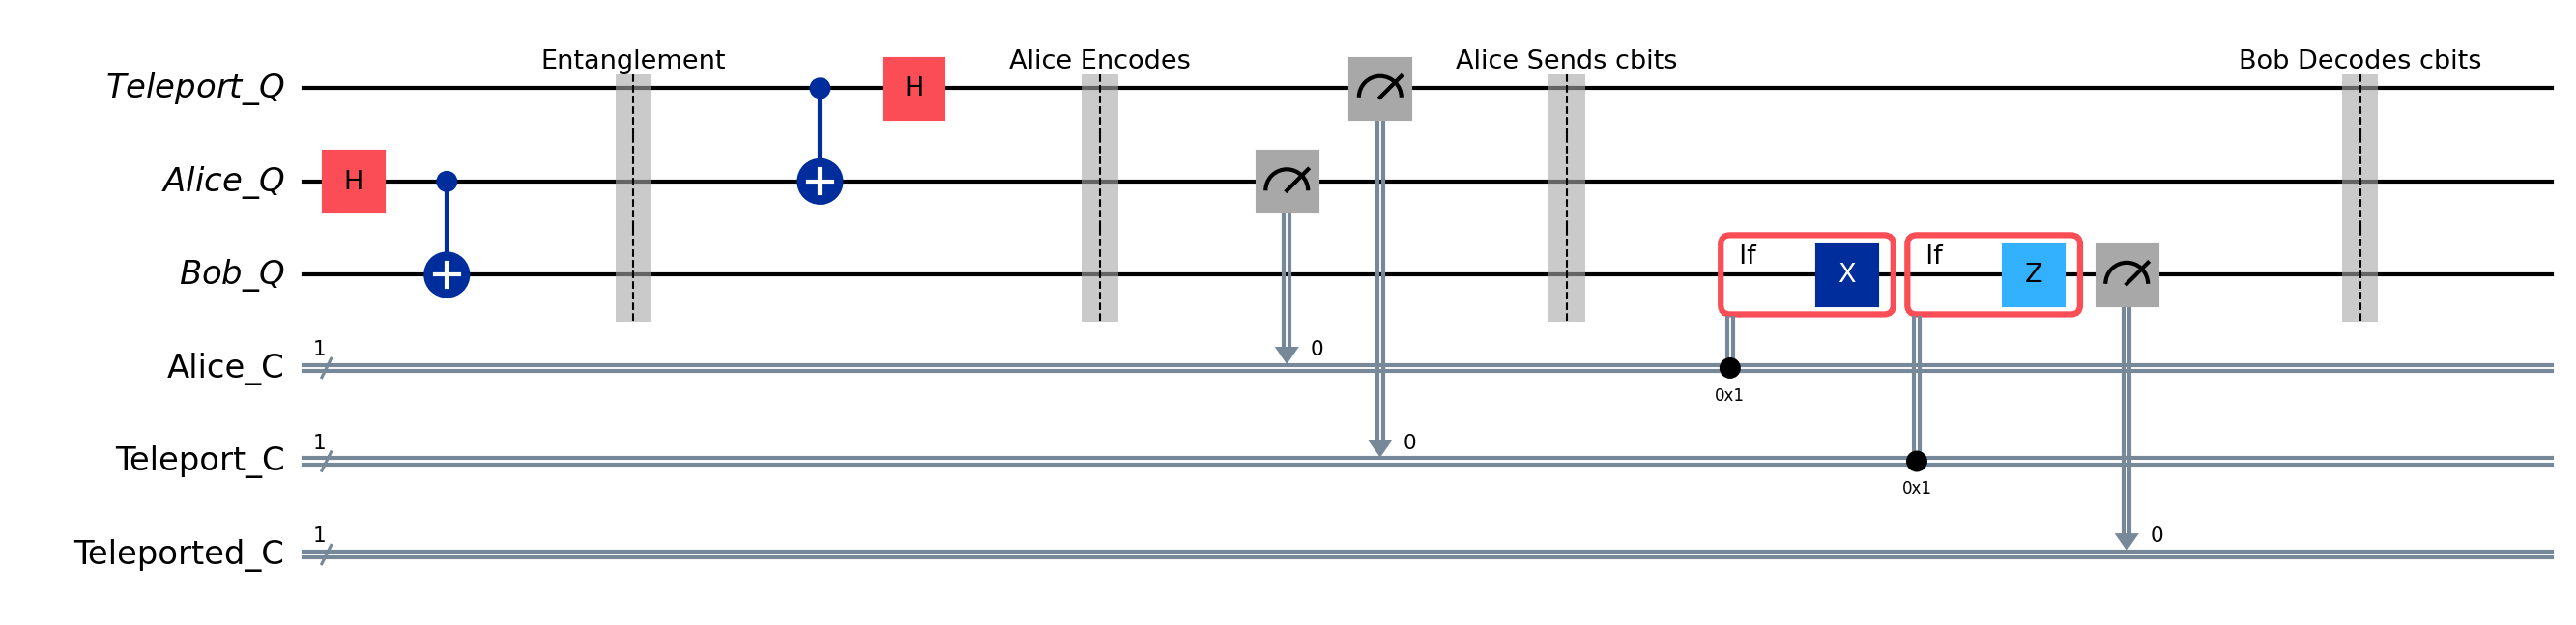
\includegraphics[width=\linewidth]{exercise3/aer_simulator__circuit.png}
    \end{minipage}
\end{figure}

\begin{figure}[h!]
    \centering
    \caption{Alice Measurements}
    \label{am}    
    \begin{minipage}{0.49\textwidth}
        \centering
        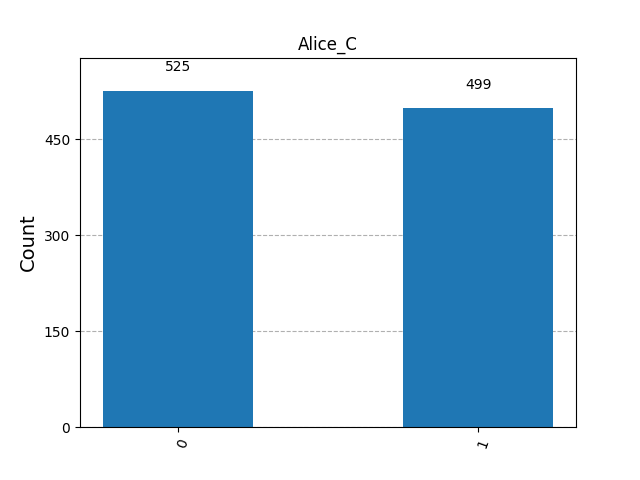
\includegraphics[width=\linewidth]{exercise3/94df8a48-88cc-4ec6-8341-d8ae773c7c37__Alice_C__counts.png}
    \end{minipage}
    \hfill
    \begin{minipage}{0.49\textwidth}
        \centering
        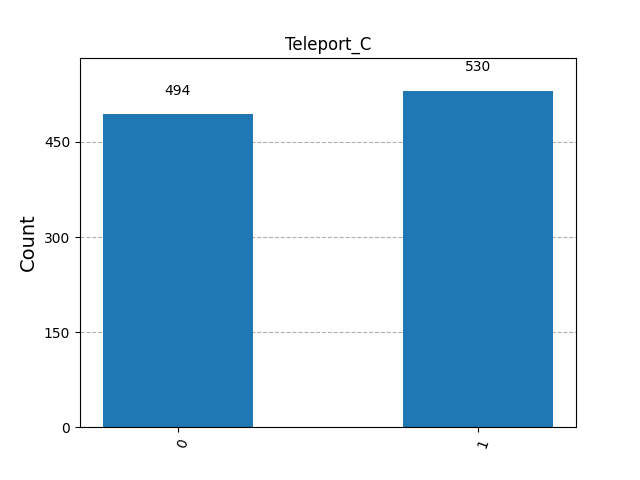
\includegraphics[width=\linewidth]{exercise3/94df8a48-88cc-4ec6-8341-d8ae773c7c37__Teleport_C__counts.png}
    \end{minipage}
\end{figure}

\begin{figure}[h!]
    \centering
    \caption{Bob Measurement of Teleported Qubit}
    \label{bm}    
    \begin{minipage}{0.49\textwidth}
        \centering
        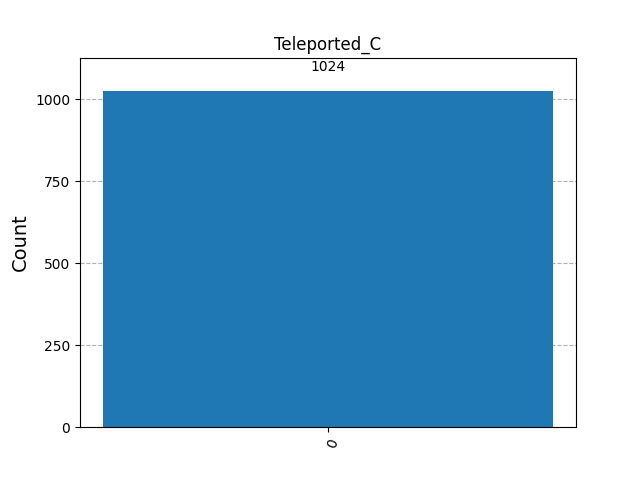
\includegraphics[width=\linewidth]{exercise3/94df8a48-88cc-4ec6-8341-d8ae773c7c37__Teleported_C__counts.png}
    \end{minipage}
\end{figure}

\vspace{6cm} % Adds 1 centimeter of vertical space

We can test the Teleportation Circuit by flipping the initial state of \textbf{Teleport\_Q} qubit, from $|0\rangle$ to $|1\rangle$, and we should expect Bob's measurement to be 1, representing the teleported state of \textbf{Teleport\_Q} to \textbf{Bob\_Q} (Fig. \ref{ctt}). We can validate the Bob's Qubit state which flipped to $|1\rangle$. The results of the measurement in Fig. \ref{am2} and Fig. \ref{bm2} bellow.

\begin{figure}[h!]
    \centering
    \caption{Circuit}
    \label{ctt}
    \begin{minipage}{1\textwidth}
        \centering
        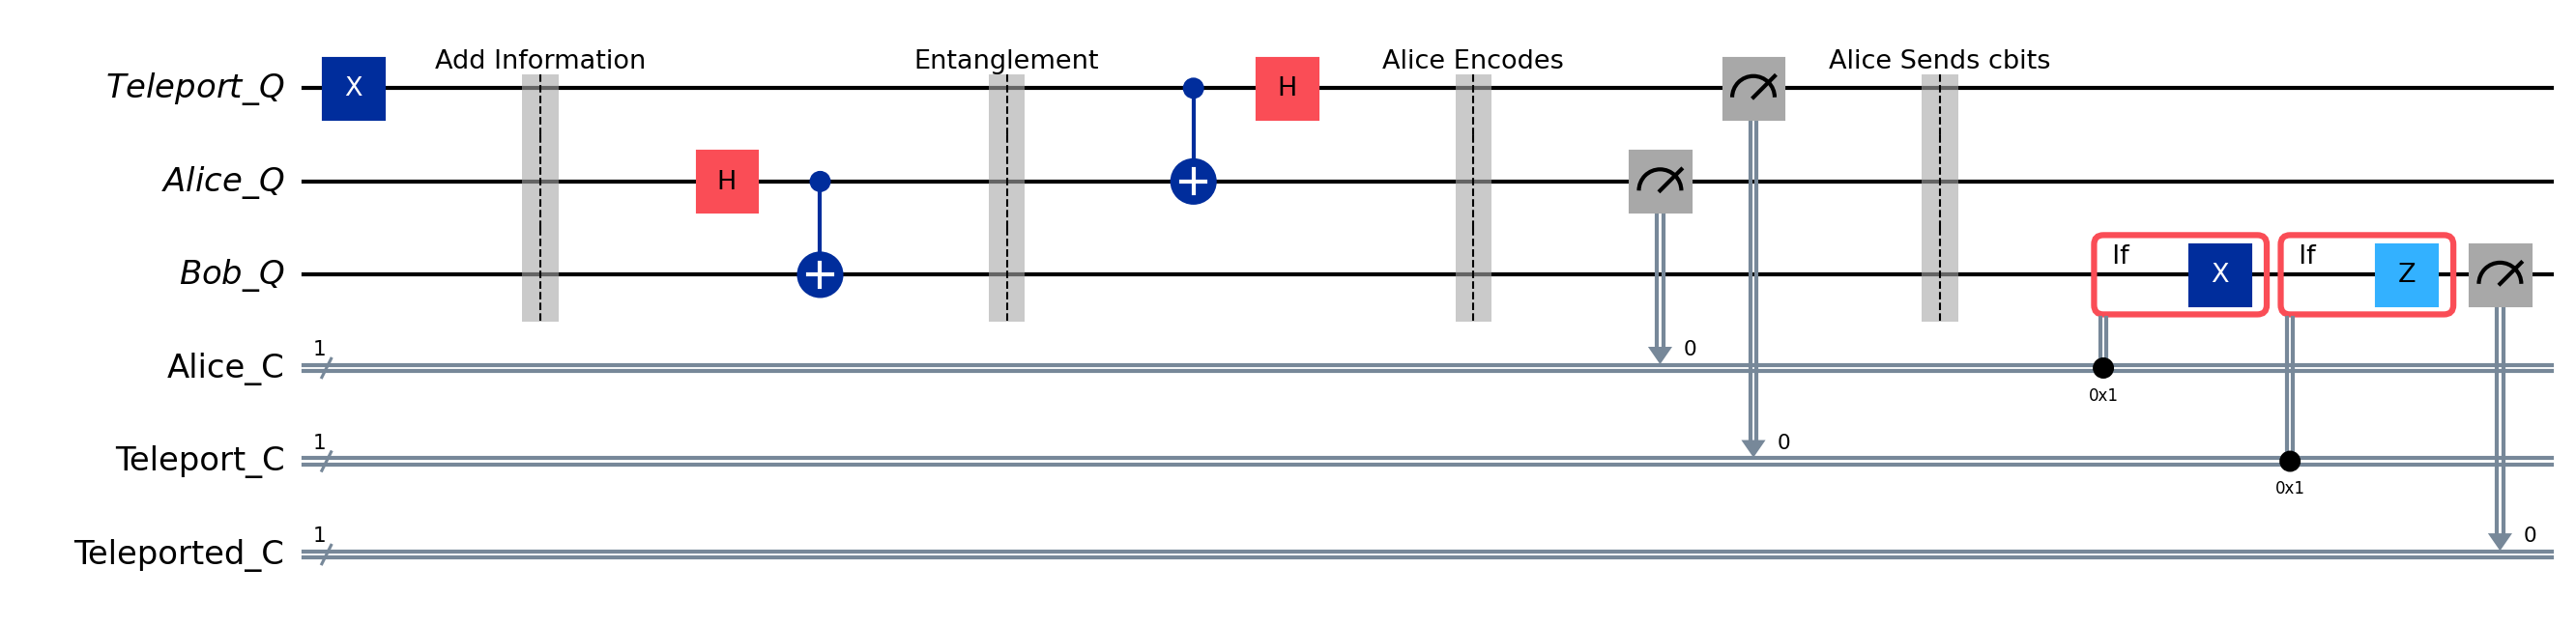
\includegraphics[width=\linewidth]{exercise3/test/aer_simulator__circuit.png}
        \caption*{aer\_simulator(fake\_brisbane)}
    \end{minipage}
\end{figure}



\begin{figure}[h!]
    \centering
    \caption{Alice Measurements}
    \label{am2}    
    \begin{minipage}{0.49\textwidth}
        \centering
        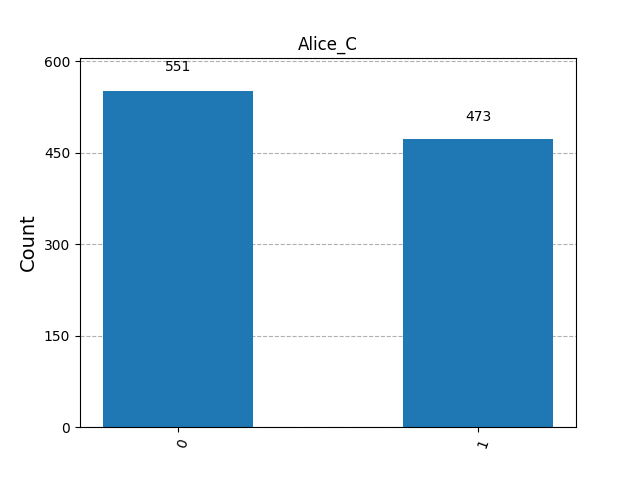
\includegraphics[width=\linewidth]{exercise3/test/51c5350c-8263-4c16-85e8-2cce2067faf0__Alice_C__counts.png}
    \end{minipage}
    \hfill
    \begin{minipage}{0.49\textwidth}
        \centering
        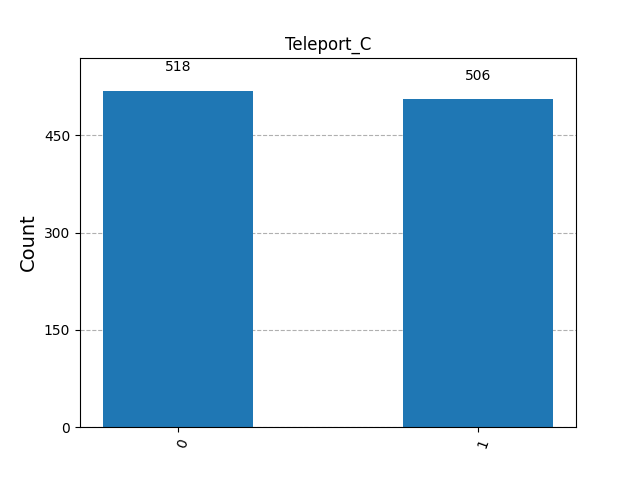
\includegraphics[width=\linewidth]{exercise3/test/51c5350c-8263-4c16-85e8-2cce2067faf0__Teleport_C__counts.png}
    \end{minipage}
\end{figure}

\begin{figure}[h!]
    \centering
    \caption{Bob Measurement of Teleported Qubit}
    \label{bm2}    
    \begin{minipage}{0.49\textwidth}
        \centering
        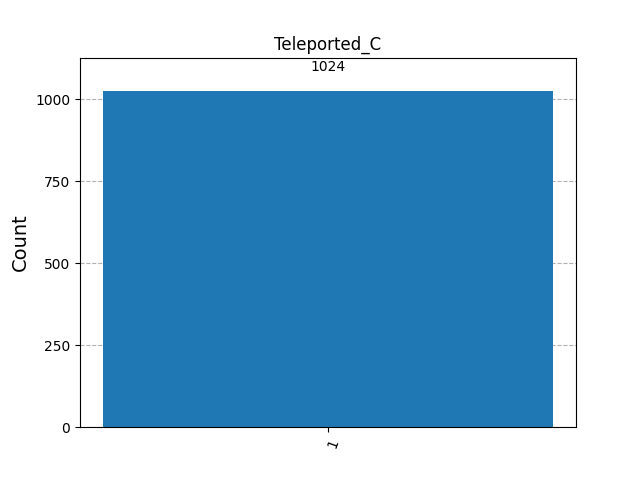
\includegraphics[width=\linewidth]{exercise3/test/51c5350c-8263-4c16-85e8-2cce2067faf0__Teleported_C__counts.png}
    \end{minipage}
\end{figure}

\vspace{5cm} % Adds 1 centimeter of vertical space


\end{document}
